
\section{Introducci�n}

\subsection{Definici�n del Problema}
\begin{frame}{Definici�n del Problema}

\framesubtitle{Reconocimiento de Actividades Humanas}
\begin{quote}
Determinar las acciones o comportamientos de uno o m�s individuos
a partir de datos ambiguos capturados por sensores situados en el
entorno.
\end{quote}
\begin{block}<2>{Nota}
\emph{}El problema es conocido por sus siglas \structure{HAR} en
ingl�s \emph{(Human Activity Recognition})
\end{block}
\end{frame}
%
\begin{frame}{Definici�n del Problema}

\setbeamercovered{transparent}

\framesubtitle{�Que es HAR?}
\begin{itemize}[<+->]
\item Es un t�pico de investigaci�n multidisciplinario que busca dise�ar
algoritmos para:
\begin{itemize}
\item Capturar movimientos de uno o m�s individuos en interacci�n con su
entorno 
\item Realizar el aprendizaje e inferencia
\item Proveer informaci�n de contexto 
\end{itemize}
\end{itemize}
\begin{overprint}
\onslide<2> 
\begin{center}
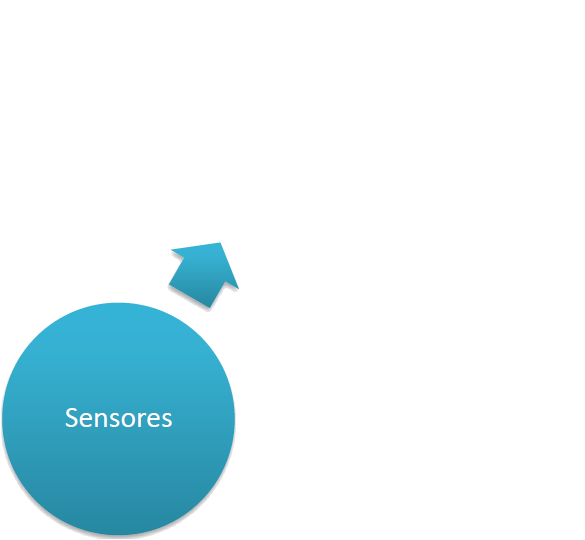
\includegraphics[width=4.5cm]{intro/graphics/areas-1}
\par\end{center}
\onslide<3> 
\begin{center}
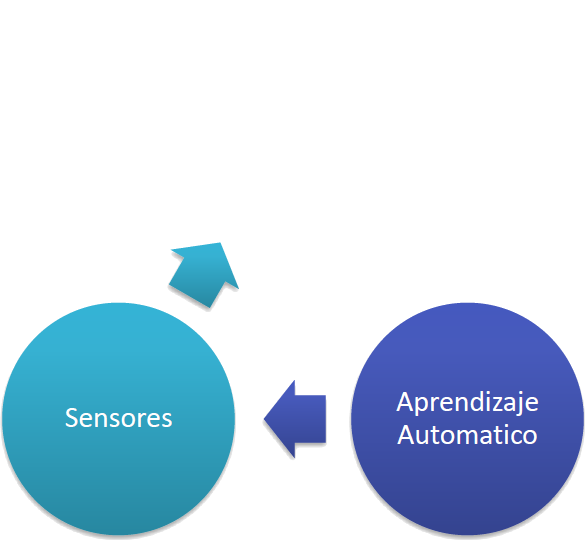
\includegraphics[width=4.5cm]{intro/graphics/areas-2}
\par\end{center}
\onslide<4> 
\begin{center}
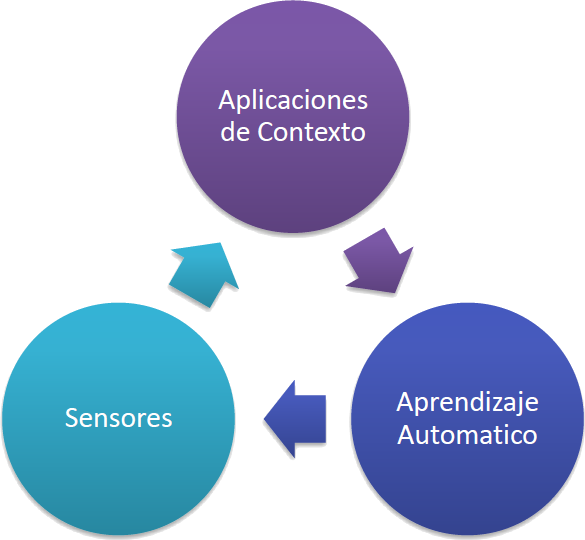
\includegraphics[width=4.5cm]{intro/graphics/areas-3}
\par\end{center}

\end{overprint}
\end{frame}
%
\begin{frame}{Definici�n del Problema}

\framesubtitle{Motivaci�n}
\begin{columns}

\column{6cm}
\begin{itemize}[<+->]
\item Reconocer el \structure{contexto} es primordial en sistemas inteligentes 
\item Avances acelerados en tecnolog�as de \structure{computaci�n m�vil}
y \structure{sensores} 
\item Uso intensivo de \structure{tel�fonos m�viles modernos} por personas
en su vida diaria.
\item \setbeamercovered{transparent}Popularidad de \structure{aplicaciones m�viles}
de contexto en �mbito de
\begin{itemize}
\item cuidado personal, 
\item la movilidad y 
\item la asistencia en la vida diaria 
\end{itemize}
\end{itemize}

\column{4cm}
\begin{overprint}
\onslide<1> 
\begin{center}
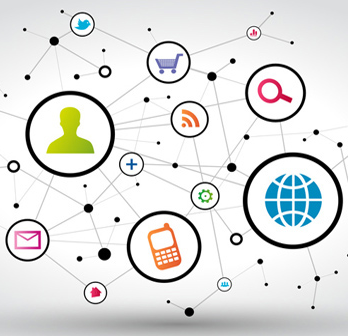
\includegraphics[width=\textwidth]{intro/graphics/context1}
\par\end{center}
\onslide<2> 
\begin{center}
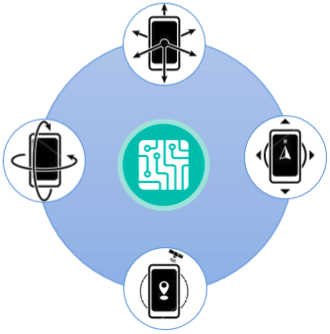
\includegraphics[width=\textwidth]{intro/graphics/sensors}
\par\end{center}
\onslide<3-> 

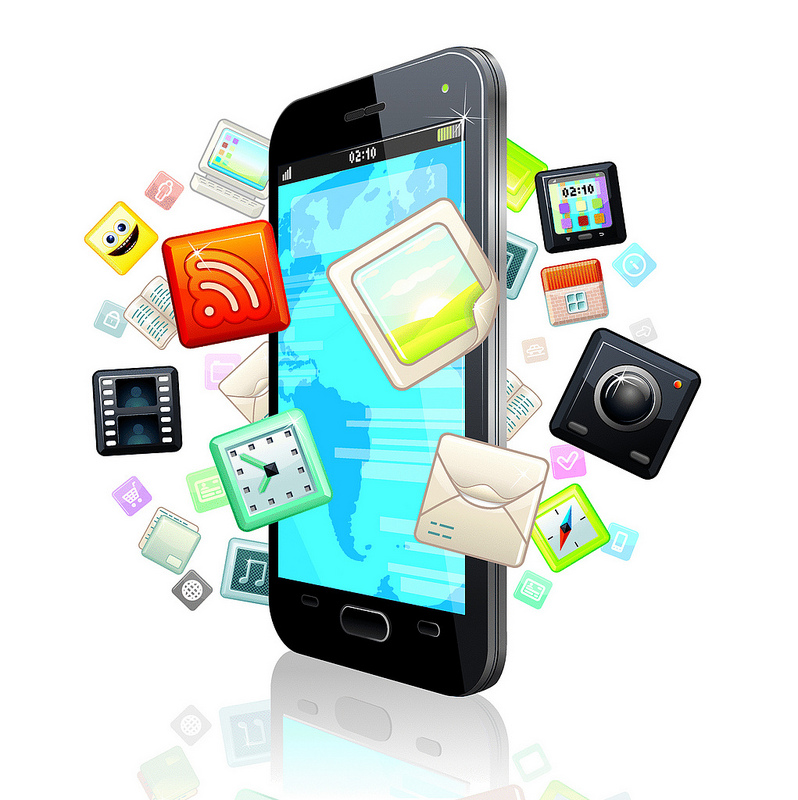
\includegraphics[width=\textwidth]{intro/graphics/mobile-phone}

\end{overprint}
\end{columns}

\end{frame}
%
\begin{frame}{Definici�n del Problema}

\framesubtitle{Actividades Humanas}

Acciones peri�dicas simples de larga duraci�n.
\begin{center}
\begin{table}
\caption{Actividades B�sicas}

\centering{}%
\begin{tabular}{|c|>{\raggedright}p{5cm}|}
\hline 
Ambulatorias & Caminar, correr, sentarse, pararse, quieto, acostarse, subir y descender
escaleras\tabularnewline
\hline 
Transporte & En bus, bicicleta y conducir\tabularnewline
\hline 
\end{tabular}
\end{table}
\par\end{center}

\end{frame}
%
\begin{frame}{Definici�n del Problema}

\framesubtitle{Actividades Humanas}

Acciones cortas o peri�dicas
\begin{center}
\begin{table}
\caption{Actividades Complejas}

\centering{}%
\begin{tabular}{|c|>{\raggedright}p{5cm}|}
\hline 
Cotidianas & Comer, beber, mirar TV, leer, cepillarse los dientes, entre otros.\tabularnewline
\hline 
Gimnasio & Alzar pesas, ejercicio aer�bico, bicicleta est�tica.\tabularnewline
\hline 
Militares & Arrastrarse, en cuclillas, irrumpir\tabularnewline
\hline 
\end{tabular}
\end{table}
\par\end{center}
\end{frame}

